\documentclass[11pt]{article}
\usepackage{url}
\usepackage{graphicx}
\usepackage{float}
\usepackage{enumerate}
\usepackage{listings}
\renewcommand{\thesection}{\Roman{section}} 
\renewcommand{\thesubsection}{\arabic{subsection}}
\title{\textbf{Generation of a 3D object from a Digital Elevation Model (DEM)}}
\author{\textbf{Supervisor: Prof. Pascal Desbarats}\\\\
		VU Manh Tu\\
		NGUYEN Bao Xuan Truong\\
		PHAM Phu Quoc\\
		BUI The Anh		
		}
\date{06-04-2016}

\begin{document}
\maketitle
\section{DEM File}
\subsection{Project overview}
This report outlines the design and development of a computer software to visualize DEM files, which are from different formats, in 3-Dimensions. It allows users using several convenient functionalities such as rotations, translation, zoom along the axises, resizing or cropping using boundary boxes, creating a support at its basis to transform it into 3D object, labeling it on. The result can be exported in OBJ and STL formats. 

The solution should be developed on \emph{C++ / Qt framework}\footnote{\url{http://http://www.qt.io/ide/}} and a visualization in \emph{OpenGL}\footnote{Opengl-superbible-comprehensive-tutorial-and-reference-5th-edition-2010}.

\subsection{Concepts}
\subsubsection{What is digital elevation model (DEM)?}
A digital elevation model (DEM) is a digital model or 3D representation of a terrain's surface — commonly for a planet (including Earth), moon, or asteroid — created from terrain elevation data.
\par\noindent It is 2D map in which each point is associated with its height. DEM can be obtained through techniques such as photogrammetry, lidar, land, surveying, etc.\footnote{\url{https://en.wikipedia.org/wiki/Digital_elevation_model}}


\subsubsection{DEM file formats}

\underline{USGS DEM}\\
The USGS DEM format is a standard format for the storage of raster digital elevation data. The USGS has produced five different digital elevation products  with the primary differing characteristic being the spacing, or sampling interval, of the data:\footnote{\url{http://agdc.usgs.gov/data/usgs/geodata/dem/dugdem.pdf}}
\begin{itemize}
\item 7.5-Minute DEM 30- x 30-meter data spacing
\item 2-Arc-Second DEM 2- x 2-arc-second data spacing
\item 15-Minute Alaska DEM 2- x 3-arc-second data spacing
\item 7.5-Minute Alaska DEM 1- x 2-arc-second data spacing
\item 1-degree DEM 3- x 3-arc-second data spacing
\end{itemize}

\noindent\textit{Purpose} 
\\ DEM file is used in the generation of three-dimensional graphics displaying terrain slope, aspect (direction of slope), and terrain profiles between selected points. At the USGS, DEMs have been used in combination with digital raster graphics (DRG's), digital line graphs (DLG's), and digital orthophoto quadrangles (DOQ's) to both enhance the visual information for data extraction and revision purposes and to create aesthetically pleasing and dramatic hybrid digital images. Non-graphic applications such as modeling terrain and gravity data for use in the search for energy resources, calculating the volume of proposed reservoirs, and determining landslide probability have also been developed.\footnote{\url{http://www.softree.com/Tips_Techniques/T-004-USGS-DEM/USGS_DEM.pdf}}
\\\\ \textit{Structure} 
\\ DEM file is an ASCII file format consisting of a header record (Type A), data records (Type B) and an accuracy metadata record (Type C)\footnote{\url{http://www.geobc.gov.bc.ca/base-mapping/atlas/trim/specs/BC-DEM-specifications-2002-12.pdf}}
\\ The physical structure of the DEM distributed to the user is as follows:\footnotemark[4]
\begin{itemize}
\item Data recorded in fixed-block format on unlabeled or ANSI-labeled 9-track magnetic tape at 1,600 or 6,250 bpi density. 
\item Logical record size of 1,024 bytes. No more than one logical record type (A, B, or C) recorded in any 1,024-byte record. However, more than one 1,024-byte record is usually required to store a single record type B. The logical record is padded with blanks if necessary to fill to the end of the 
logical record. Bytes 1,021-1,024 of each logical record are padded with blanks. 
\item Physical record size of 4,096 bytes; that is, 4 logical records per physical record. 
\item Data written as ANSI-standard ASCII characters.
\end{itemize}

\noindent \underline{SDTS DEM}\\
SDTS stands for Spatial Data Transfer Standard, is a robust way of transferring earth-referenced spatial data between dissimilar computer systems with the potential for no information loss. It is a transfer standard that embraces the philosophy of self-contained transfers, i.e. spatial data attribute, dereferencing, data quality report, data dictionary, and other supporting metadata all included in the transfer. \footnote{\url{http://mcmcweb.er.usgs.gov/sdts/whatsdts.html}}\\ 
SDTS has 7 parts. Parts 1-3 are about SDTS specification which is organized into the base specification, all of them are related, but relatively independent. Parts 4-6 are about multiple profiles, each define specific rules and formats for applying SDTS for the exchange of particular types of data in SDTS: \footnote{\url{http://mcmcweb.er.usgs.gov/sdts/standard.html}}
\begin{itemize}
\item Part 1 – Logical Specifications:
\par\noindent It consists of three main sections, which explain the SDTS conceptual model and SDTS spatial object types, components of a data quality report, and the layout of all SDTS modules.
\item Part 2 – Spatial Features: 
\par\noindent It contains a catalogue of spatial features and associated attributes. This part addresses a need for definition of common spatial feature terms to ensure greater compatibility in data transfers. The current version of Part 2 is limited to small- and medium-scale spatial features commonly used on topographic quadrangle maps and hydrographic charts.
\item Part 3 – ISO 8211 Encoding: 
\par\noindent This part explains the use of a general purpose file exchange standard, ISO 8211, to create SDTS file sets (i.e. transfers).
\item Part 4 - Topological Vector Profile:\\
The Topological Vector Profile (TVP) is the first of a potential series of SDTS profiles, each of which defines how the SDTS base specification (Parts 1, 2, and 3) must be implemented for a particular type of data. The TVP limits options and identifies specific requirements for SDTS transfers of data sets consisting of topologically structured area and linear spatial features.
\item Part 5 - Raster Profile and Extensions: 
\par\noindent The Raster Profile is for 2-dimensional image and gridded raster data. It permits alternate image file formats using the ISO Basic Image Interchange Format (BIIF) or Dereferenced Tagged information File Format (Geo TIFF).
\item Part 6 - Point Profile: 
\par\noindent The Point Profile contains specifications for use with geographic point data only, with the option to carry high precision coordinates such as those required for geodetic network control points. This profile is a modification of Part 4, the Topological Vector Profile, and follows many of the conventions of that profile.
\end{itemize}

\noindent \underline{DTED}\\ 
DTED is a standard of digital datasets which consists of a matrix of terrain elevation values \footnote{\url{https://en.wikipedia.org/wiki/DTED}}. It is the oldest digital mapping format that we still use today. This standard was originally developed in the 1970s by NIMA - the National Imagery and Mapping Agency. DTED was originally developed to drive 3D milling machines and provide elevation data needed for cruise missile planning. \footnote{\url{http://www.mission-planning.com/DTED_Part1.htm}}\\ 
DTED format have 3 level:\footnote{\url{http://fas.org/irp/program/core/dted.htm}}
\begin{itemize}
\item Level 0 
\begin{itemize}
\item Has a post spacing of approximately 900 meters.
\item Elevation post spacing is 30 arc second 
\item Derived from NIMA DTED Level 1 to support a federal agency requirement
\item DTED Level 0 may be of value to scientific, technical, and other communities for and applications that require terrain elevation, slope, and/or surface roughness information. It allows a gross representation of the Earth's surface for general modeling and assessment activities. Such reduced resolution data is not intended and should not be used for automated flight guidance or other precision activity involving the safety of the public.
\end{itemize}
\item Level 1 
\begin{itemize}
\item Has a post spacing of approximately 90 meters.
\item A uniform matrix of terrain elevation values with post spacing every 3 arc seconds
\item The information content is approximately equivalent to the contour information represented on a 250,000 scale map.
\end{itemize}
\item Level 2 
\begin{itemize}
\item Has a post spacing of approximately 30 meters. 
\item He basic high resolution elevation data source for all military activities and systems that require landform, slope, elevation, and/or terrain roughness in a digital format.
\end{itemize}
\end{itemize}

\noindent \underline{DIMAP}\\
The DIMAP stands for Digital Image Map. It is the format for SPOT products introduced for the SPOT 5 launch in May 2002 and developed with CNES.\footnotemark \\
DIMAP format consists of two parts:\footnotemark[\value{footnote}]
\footnotetext{\url{http://www.geo-airbusds.com/en/196-the-dimap-format}}
\begin{itemize}
\item Image: By default it is described in GeoTIFF format, comprised of
\begin{itemize}
\item A TIFF part, the most widely used image format in the world.
\item A Geo part, adding georeferencing information for the image file (coordinates in the upper left-hand corner of the image and pixel size) to the basic TIFF file and may also describe the map projection used and its corresponding geographic system.
\end{itemize}
\item Metadata: this is written in XML, allowing to create customized keywords with corresponding values. It can be linked to an XSL style sheet which sorts and does the HTML layout of the information contained in the XML file.
\end{itemize}

\section{Software requirements}
\subsection{Functional requirements}
\subsubsection{Functional requirement 1}
\begin{itemize}
\item ID: FR1
\item TITLE: Install application
\item DESC: A user has downloaded the application, then he should be able to install this application by following the instruction.  After install, the application must notification if install success or not.
\item RAT: In order for a user to install application.
\item DEP: 
\end{itemize}
\subsubsection{Functional requirement 2}
\begin{itemize}
\item ID: FR2
\item TITLE: Select DEM file to open
\item DESC: After the installation, the user should be able to run it and open file to import. The application must show 3D image of imported file if its format is acceptable.Otherwise, it shows notification that the file format is incorrect.
\item RAT: For a user to open DEM file and visualize it in 3D
\item DEP: FR1
\end{itemize}
\subsubsection{Functional requirement 3}
\begin{itemize}
\item ID: FR3
\item TITLE: Rotate a 3D Image
\item DESC: After having a 3D Image, then the user should be able to rotate it by using mouse movement action. The rotation includes move up, down, left, right or any angles
\item RAT: For a user to rotate 3D image.
\item DEP: FR2
\end{itemize}
\subsubsection{Functional requirement 4}
\begin{itemize}
\item ID: FR4
\item TITLE: Zoom in/out a 3D Image
\item DESC: After having a 3D Image, the user should be able to zoom in the 3D image by double clicking mouse. The mouse clicked point must be in range of 3D image. The user is also able to zoom out the 3D image by hold CRTL key while click.
\item RAT:For a user to zoom in/out 3D image.
\item DEP: FR2
\end{itemize}
\subsubsection{Functional requirement 5}
\begin{itemize}
\item ID: FR5
\item TITLE: Select an area in a 3D Image
\item DESC: After having a 3D Image, the user should be able to select an area in 3D Image by using mouse to draw a box on the 3D Image
\item RAT: For a user to select an area in 3D image.
\item DEP: FR2
\end{itemize}
\subsubsection{Functional requirement 6}
\begin{itemize}
\item ID: FR6
\item TITLE: Resize an area in boundary box in a 3D Image
\item DESC: Given that a user has selected an area on 3D Image, then the user should be able to resize this area by clicking right mouse and select resize. A dialog must show in order to select how many percentage will be resized.
\item RAT: For a user to resize an area in a 3D image.
\item DEP: FR5
\end{itemize}
\subsubsection{Functional requirement 7}
\begin{itemize}
\item ID: FR7
\item TITLE: Crop a boundary box on 3D Image
\item DESC: Given that a user has selected an area on 3D Image, then the user should be able to crop this area by clicking right mouse and select crop. After cropped, only the area within boundary box remains.
\item RAT: For a user to crop an area in 3D image.
\item DEP: FR5
\end{itemize}
\subsubsection{Functional requirement 8}
\begin{itemize}
\item ID: FR8
\item TITLE: Create a support at the basis of 3D image
\item DESC: After having a 3D Image, the user should be able to create a support at the basis of current 3D image by clicking the "Create support" button. With the support, the 3D object should be ready to be printed by a 3D printer.
\item RAT: In order for user to transform image into 3D object.
\item DEP: FR2
\end{itemize}
\subsubsection{Functional requirement 9}
\begin{itemize}
\item ID: FR9
\item TITLE: Label the 3D object
\item DESC: Given that a user has created a support at the basis of 3D image. The user should be able to label the 3D object by clicking the "Text" button, then clicking a position on the object or at its support to create textbox where user can write some note as label.
\item RAT: For user to label the 3D object
\item DEP: FR8
\end{itemize}
\subsubsection{Functional requirement 10}
\begin{itemize}
\item ID: FR10
\item TITLE: Export to OBJ, STL files
\item DESC: Given that a user has created 3D object, and may or may not be has labeled it. The user should be able to export to OBJ or STL file by clicking the "Export" button. 
\item RAT: For user to export to OBJ, STL files
\item DEP: FR8
\end{itemize}
\subsection{Non-functional requirements}
\begin{itemize}
\item Compatible operation system: Linux
\item Operation fluidity: Rotate, translate, zoom, resize, crop 3D image, create support at its basis or label the object should be executed without delay. 
\end{itemize}

\section{Architecture Design}
\subsection{Introduction}
\subsubsection{Purpose}
This part will explain the architecture of the application.
\subsubsection{ Developing environment}
\begin{itemize}
\item OS: Linux
\item Framework: QT(QT quick QML).
\item 3D render library: OpenGL.
\end{itemize}

\subsubsection{Usability \& Maintenance}
\indent We use design pattern MVC for this project. MVC (Model–View–Controller) is a software architectural pattern for implementing user interfaces on computers. It divides a given software application into three interconnected parts, so as to separate internal representations of information from the ways that information is presented to or accepted from the user. In the Model modules we have File Data Object and I/O Layer. The Controller modules we have 3D Process, Modules Process and Control View Data (This part going to contact to View modules, for what you wait to show) all of them for processing DEM files, how to move, cut, and zoom 3D image and print 3D object. Finally is View modules. this is only show the data from the Control View Data, and it has the UI in which user easily contact to the Controller Modules.
\break
\indent Why do we use the design above? First, it is about usability, which means the developers will know where and what they need to look into with specific situation. When a problem happens, developers can detect where the problems are and what to do next. For example, if we have a problem about zoom DEM images, that means we know the problem from Zoom modules and this modules has a problem from Zoom Controller. The developers read the zoom method and fixes the wrong algorithm. They can easily make more features without care about other modules. Finally, it is so easy for maintenance, not only for us, but also other teams if they are going to reuse our code. Because, although it has many modules, we only have to maintain the module that has problems.
\break

\subsection{Overall Description}
\subsubsection{System architecture}
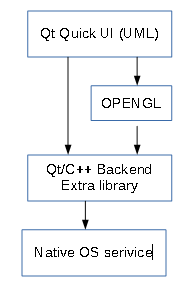
\includegraphics{1.png}
\begin{itemize}
\item Qt Quick (QML) framework: Build user interface. Handling binding data, view animation.
\item OPENGL: Provide 3D process library.
\item Qt/C++: Provide database, file access api.
\item Extra library: library for processing dem file.
\end{itemize}

\subsubsection{Software block diagram}
\noindent\makebox[\textwidth]{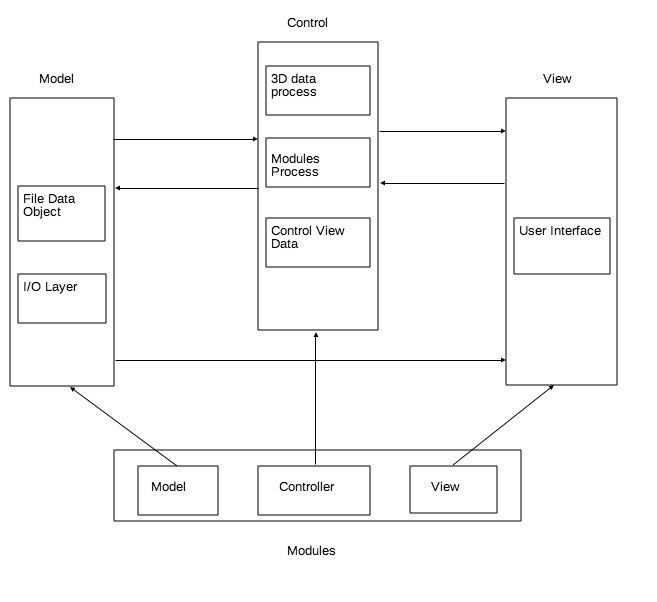
\includegraphics[width=\textwidth]{2.jpg}}
\begin{itemize}
\item Model: Handle File In/Out including read Dem file or Export. Model also holds Dem file Object
\item Controller: Control data flow, process action request from View
\item View: Show user interface
\item Modules: A component include Model, Controller \& View as part of program such as file module or zoom module
\end{itemize}

\subsubsection{Data flow}
\begin{itemize}
\item Open DEM file button
\par\noindent\makebox[\textwidth]{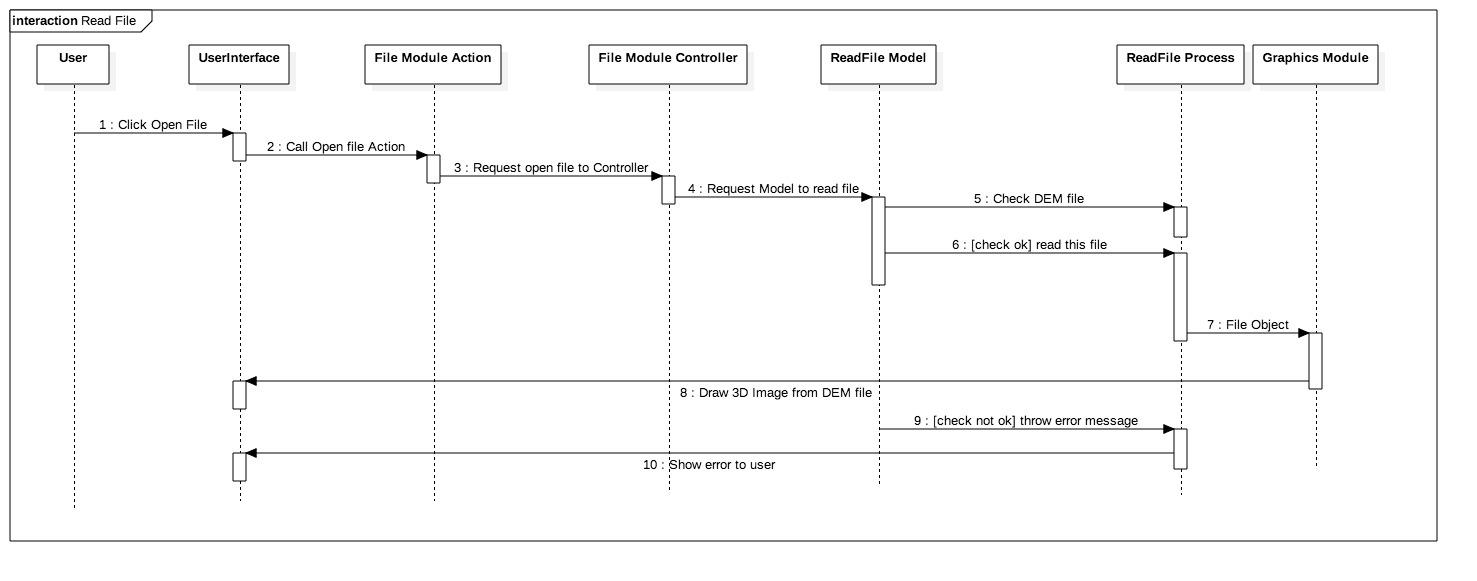
\includegraphics[width=0.9\paperwidth]{3.jpg}}
\item Zoom
\par\noindent\makebox[\textwidth]{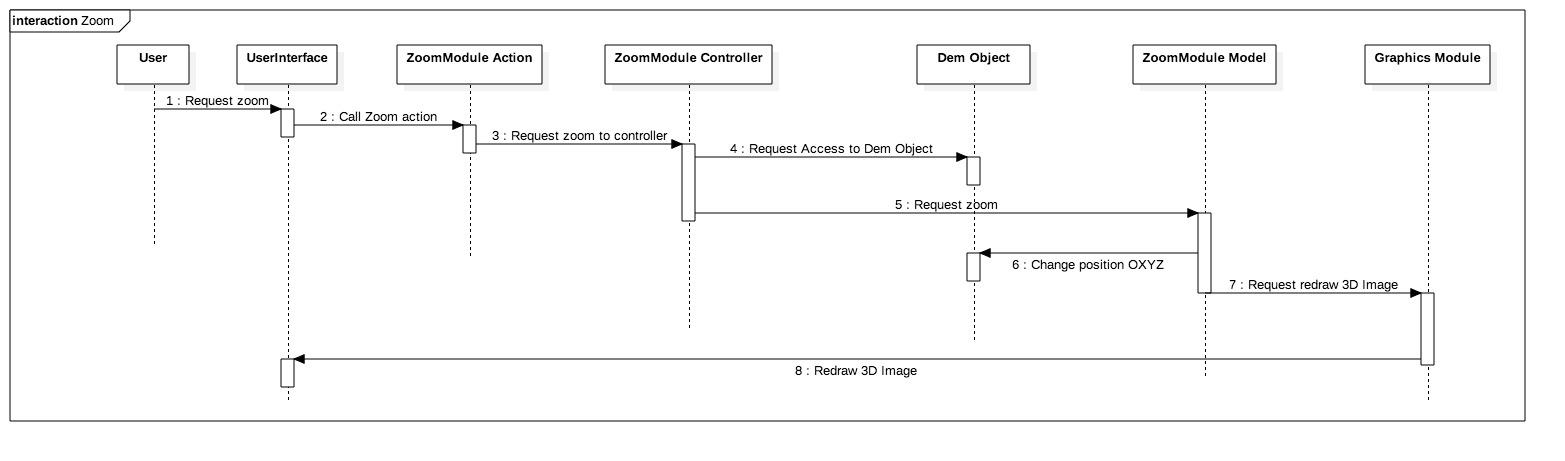
\includegraphics[width=0.9\paperwidth]{4.jpg}}
\end{itemize}

\subsubsection{Class diagram}
The main idea here is separate the program into multiple modules, each module only take care one task. For example, file module will handle reading Dem file or exporting to OBJ/STL format. To do that, we need to build a basic system with ability of adding more modules. The following class diagram provide a way to do it.
\begin{itemize}

\item Controller
\par\noindent\makebox[\textwidth]{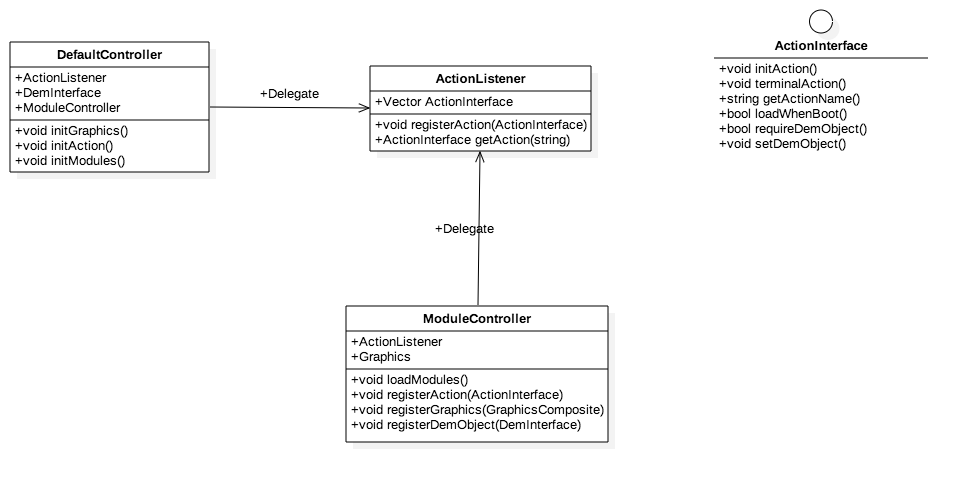
\includegraphics[width=0.9\paperwidth]{5.png}}
Action listener is the heart of the program. It provides a way for user to interact with the program. ActionListener will collect actions registered from modules \& can be called from graphic viewer if needed. ActionListener also allows modules to register to access data from model.

\item Base Element of DEM file
\par\noindent\makebox[\textwidth]{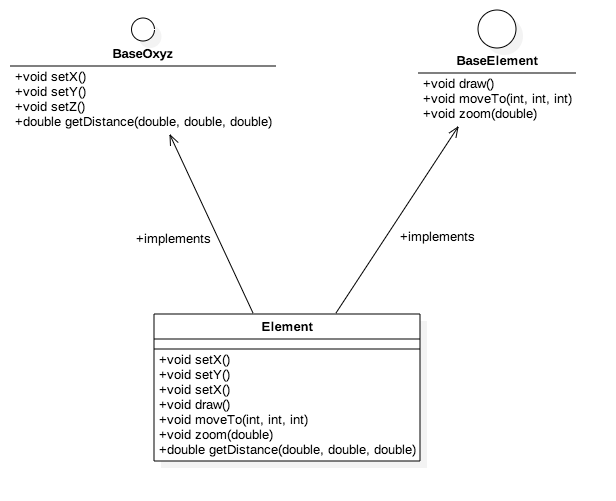
\includegraphics[width=\textwidth]{6.png}}
This is the basic element to represent element in Dem file.

\item Read DEM file
\par\noindent\makebox[\textwidth]{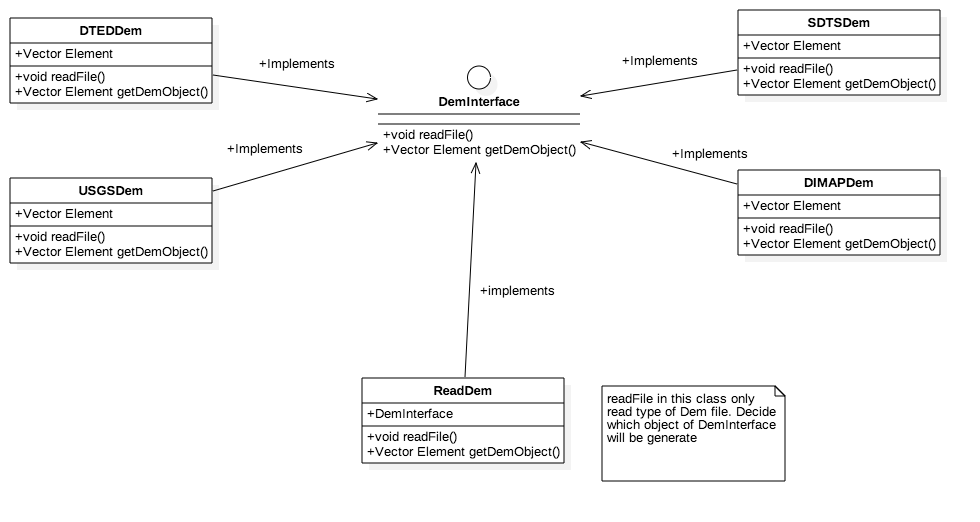
\includegraphics[width=0.9\paperwidth]{7.png}}
We have 4 types of Dem file. So, we need 4 types of class to read those types. But all of those types will have the same Dem Interface. 

\item Graphics 
\par\noindent\makebox[\textwidth]{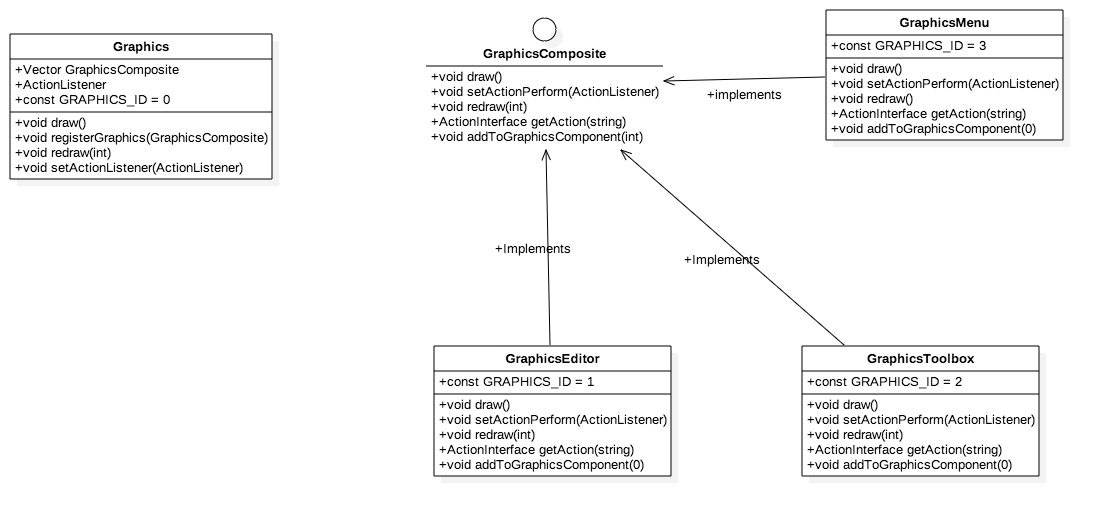
\includegraphics[width=0.9\paperwidth]{8.png}}
In the User Interface, we have 3 basic graphics component includes: 
\\GraphicsMenu: Menu in the top of program. Included a direct way to access functions of program, such as file, view, etc.
\\GraphicsToolbox: A control panel of program. 
\\GraphicsEditor: An area where 3D Image will be paint.
\item Modules
\par\noindent\makebox[\textwidth]{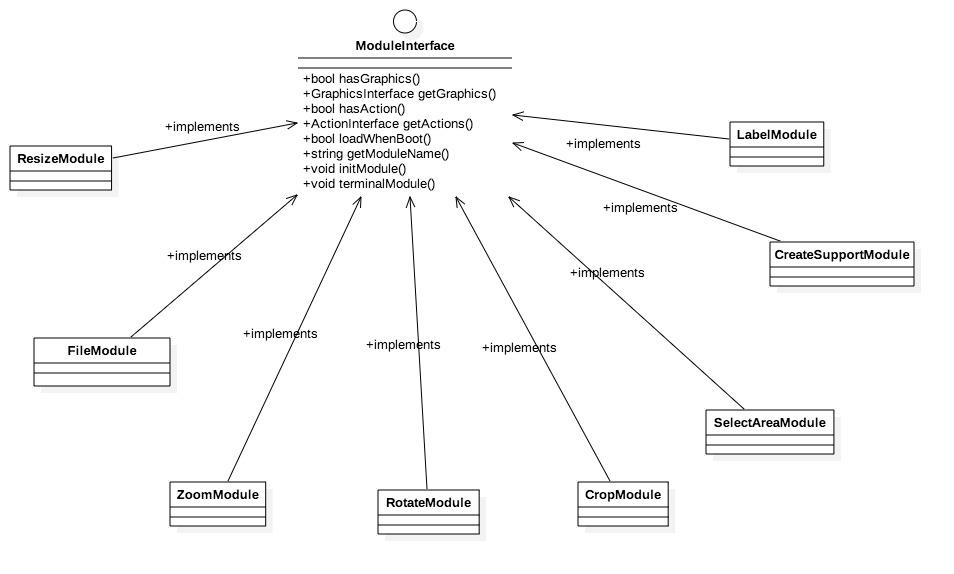
\includegraphics[width=0.9\paperwidth]{9.jpg}}
Every module in this program must implements this interface, to register a module.
\end{itemize}

\section{Test cases}
\par\makebox[\textwidth]{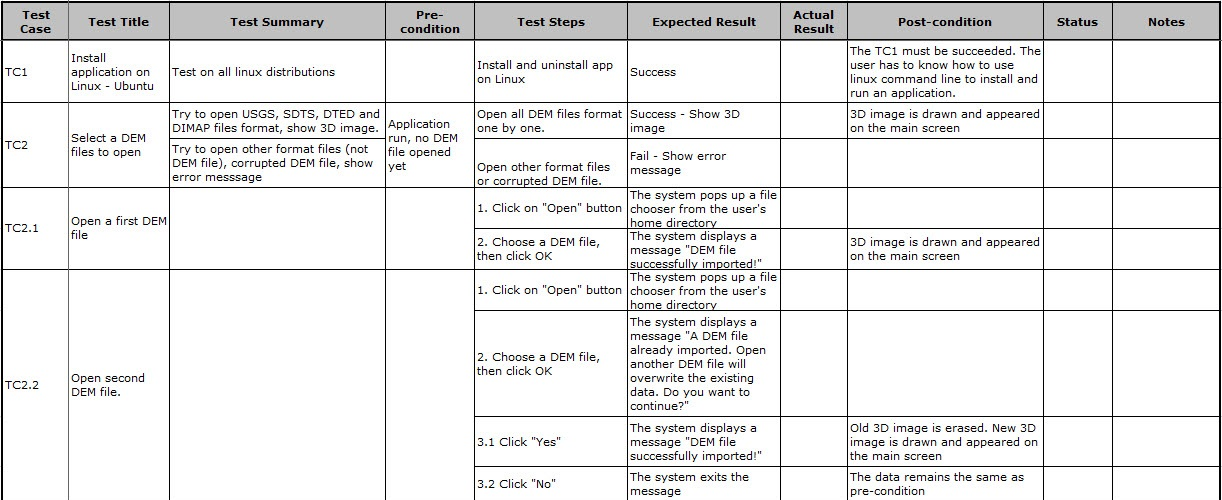
\includegraphics[width=0.9\paperwidth]{TC_P1.jpg}}
\makebox[\textwidth]{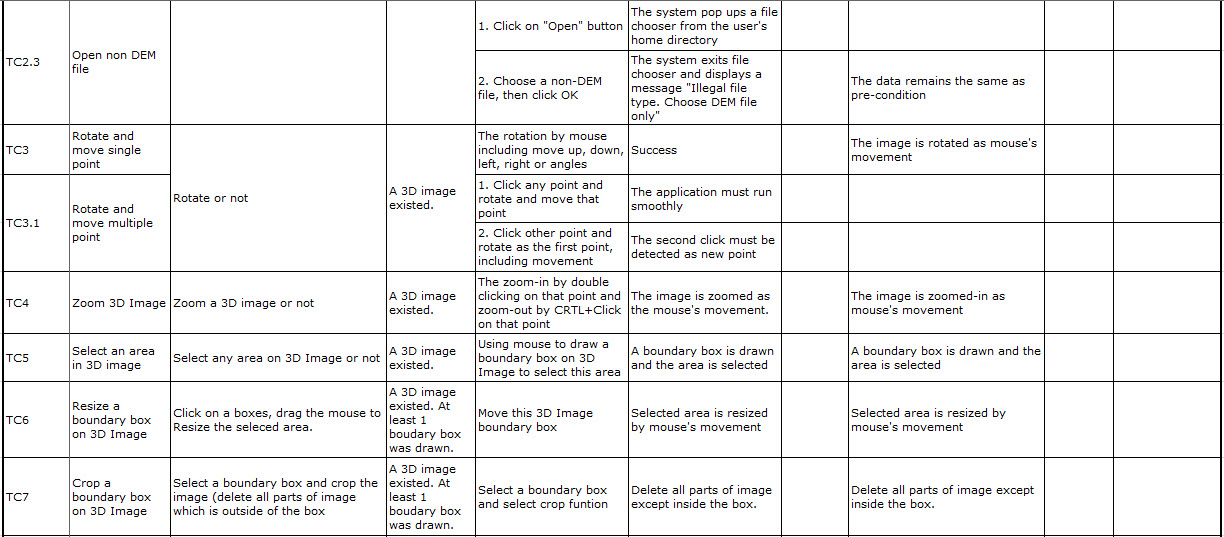
\includegraphics[width=0.9\paperwidth]{TC_P2.jpg}}
\makebox[\textwidth]{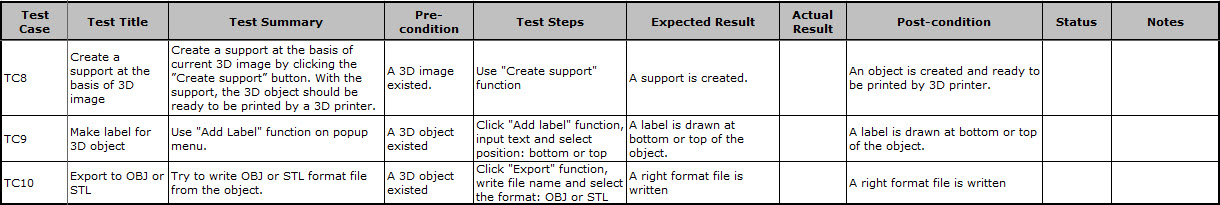
\includegraphics[width=0.9\paperwidth]{TC_P3.jpg}}
\section{Tasks assignments}
The software engineering project is scheduled with milestones:
\begin{enumerate}
\item 15 April: Report on Bibliography, existing analysis
\item 6 May: Report on Requirement analysis and objective
\item 3 June: Architecture and tests: First report completion
\item 26 August: Development: Final report
\end{enumerate}

\par\noindent The project duration is 5 months, starting at 6 April and ending at 26 August.
\par\noindent We consider to choose the Waterfall model (see figure below) to manage this project because: 
\begin{itemize}
\item The time is short: despite the official duration of 5 months, we only have about 2-3 months to work on project due to the overlapping schedules of university and/or companies.
\item The requirements are quite clear and fixed.
\item The software is not too complex.
\end{itemize}
\begin{figure}[H] 
  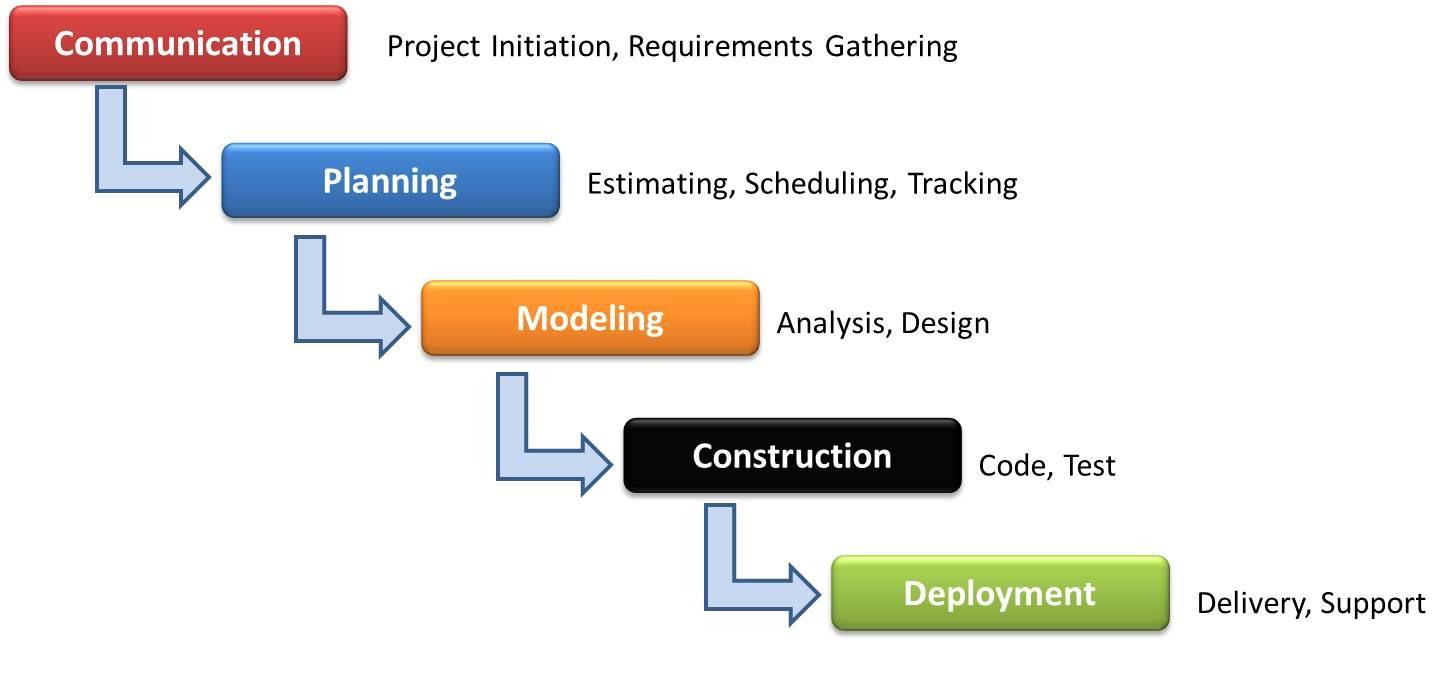
\includegraphics[width=\linewidth]{P3.jpg}
  \label{fig:wmodel}
\end{figure}
\par\noindent The following figures of Task list and Gantt chart shows how the project is controlled and tasks are organized in the team.
\begin{figure}[H] 
  \makebox[\textwidth]{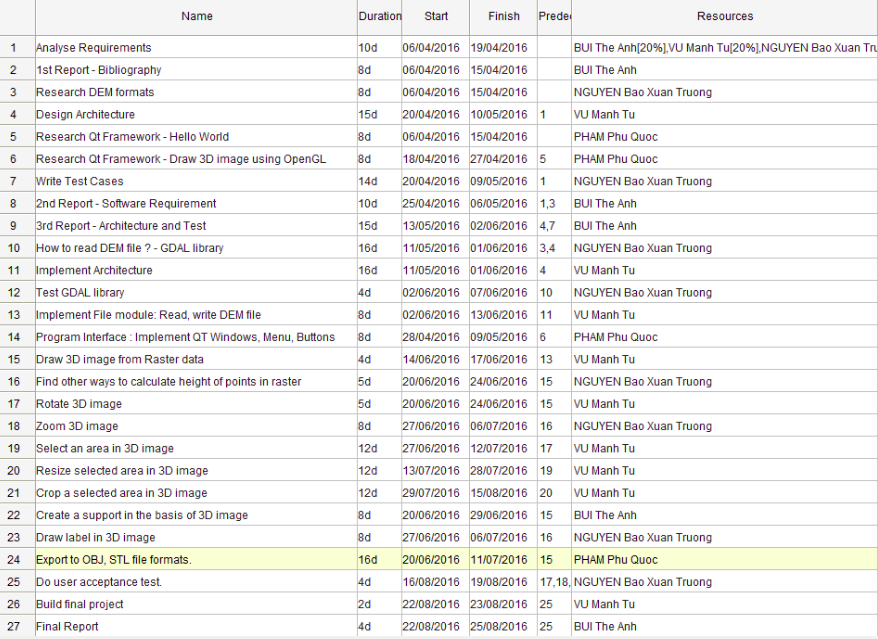
\includegraphics[width=0.6\paperwidth]{Tasks.png}}
  \label{fig:Tasks}
\end{figure}

\begin{figure}[H] 
  \makebox[\textwidth]{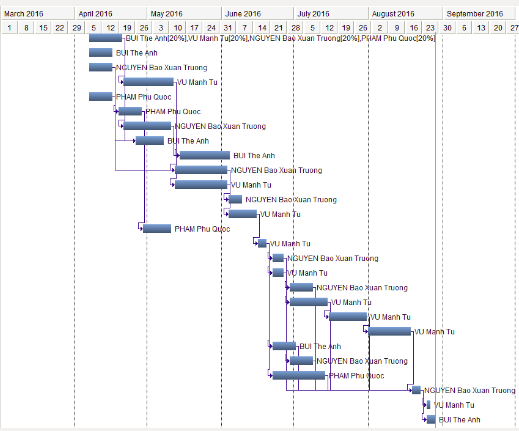
\includegraphics[width=0.9\paperwidth]{Gantt.png}}
  \label{fig:Gantt}
\end{figure} 

\section{Implementation}
\subsection{Structure Overview} 
Application is divided into modules. Each module handle a different task.
All modules have to be implemented main module file which inherits from Module Interface

\begin{lstlisting}
class ModuleInterface
{
public:
    virtual bool hasGraphics() = 0;
    virtual GraphicsComposite* getGraphic() = 0;
    virtual bool hasAction() = 0;
    virtual ActionInterface* getAction() = 0;
    virtual bool loadOnBoot() = 0;
    virtual QString getModuleName() = 0;
    virtual void initModule() = 0;
    virtual void terminalModule() = 0;
};
\end{lstlisting}

Module can have Graphics or Action depending on the property of that module. If using Graphics, it is needed to inherit from GraphicsComposite abstract class and declare in the system (method hasGraphics returns true). 

\begin{lstlisting}
class GraphicsComposite
{
protected:
    GraphicsComposite* graphicsMain;
    vector<GraphicsComposite*> graphics;
    ActionListener* actions;
    vector<Menu*> menus;
    const int GRAPHICS_ID = -1;
    DemInterface* demObject;

public:
    void setMainGraphics(GraphicsComposite*);
    GraphicsComposite* getMainGraphics();
    void setActionPerform(ActionListener* action);
    ActionInterface* getAction(QString);
    void registerGraphics(GraphicsComposite* graphic);
    int addToGraphicsComponent();
    bool addMenu(QString menuName, QAction *action);
    bool registerMenu(QMenuBar*);
    virtual void setSize(int width, int height);
    virtual void updateGraphics();
    virtual void updatePaintGL();
    QAction* createQAction( QString name );
    virtual void addVertex(Vertex vertex, int col, int row);
    void setDemObject(DemInterface* dem);
    virtual QSize getSize();
    virtual void mousePressEvent(QMouseEvent *event);
    virtual void mouseMoveEvent(QMouseEvent *event);
    virtual void mouseDoubleClickEvent(QMouseEvent *event);
    virtual void initial() = 0;
    virtual void initializeGL() = 0;
    virtual void paintGL() =0 ;
    virtual void resizeGL(int width, int height) = 0;
};
\end{lstlisting}

Abstract Graphics Composite provides basic functions for the module to interact with system. For example, to create new menu, the module only calls: 
bool addMenu(QString menuName, QAction *action);  

Similarly, if using Action, it is needed to inherit from Action Interface and declare in the system.

\begin{lstlisting}
class ActionInterface
{
private:
    ActionListener* actionPerform;
public:
    virtual void initAction() = 0;
    virtual void terminalAction() = 0;
    virtual QString getActionName() = 0;
    virtual bool loadOnBoot() = 0;
    virtual bool requireDemObject() = 0;
    virtual void setDemObject(DemInterface*) = 0;
    virtual DemInterface* getDemObject()=0;
    virtual void setGraphics(GraphicsComposite*)=0;
    virtual void setActionPerform(ActionListener*) =0;
};
\end{lstlisting}

For modules using DEM data, they must have Action. In Action, it must register to use DEM data(requireDemObject function returns true) and system will automatically provide DEM data via DemInterface.

\subsection{Modules} 
\begin{itemize}
\item a. Module Files:
Module Files creates a menu to choose DEM file, read DEM file and generate mesh.
It uses GDAL library to read DEM file into Raster data.
Raster data is an array of float type which contains height data of each pixel. Based on Raster data and number of cols, rows of DEM file, there is a 2-dimensions array.

From here, 2-dimensions array's data is changed to Frame of reference of OpenGL with center is base coordinate.
\begin{figure}[H] 
  \makebox[\textwidth]{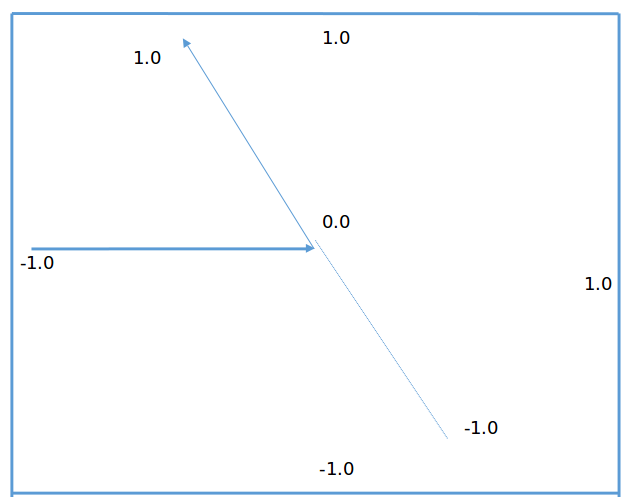
\includegraphics[width=0.5\paperwidth]{Base.png}}
  \label{fig:Base}
\end{figure} 
Calculate x,y coordinates from 2-dimensions array into frame of reference of OpenGL:

NewX = (X – CenterX)/CenterX
NewY = (CenterY - Y)/CenterY

X,Y is coordinates in 2-dimensions array.
NewX, NewY : coordinates in frame of reference in OpenGL.
CenterX : cols/2
CenterY: rows/2

\begin{lstlisting}
Code: 
for (int k = 0; k < rows; k=k+step) {
            posY = (float)(centerY - k)/centerY;
            for (int j =0; j < cols; j=j+step) {
                posX = (float)(j - centerX)/centerX;
\end{lstlisting}

For Z (height) dimension, the height in 2-dimensions is between -11000 to 9000. However,  9000 is too big to differentiate low/high positions in 3D drawing. Hence, using average = 6000.

NewZ = Data2D[X,Y]/6000;

After identifying coordinates in frame of reference of OpenGL, 3D-interpolating by using triangle:

From each point (x,y), find 4 next points: [(y+1, x), (y, x +1)] and [(y-1, x), (y, x-1)] which create 2 triangles, continue for all points in the array.

Identify normal vector: 
Normal vector is used to identify the direction of light source illuminating the terrain. Based on it, identify dark or light points in the terrain.

It is needed to identify normal vector for each vertex in mesh. When calculate 3 points  to draw a triangle, normal vector of that triangle. This vector normal will be assigned to vertices of triangle.
When 2 triangles have the same vertex, normal vector of that vertex is the combination of normal vectors of 2 triangles.
\begin{lstlisting}[breaklines=true]
void DemObject::addVertex(Vertex vertex, int position)
{
    int currentPosition = vertexs.size() - 1;
    if (position > currentPosition) {
        vertexs.push_back(vertex);        
    } else {
        vertexs[position].setNormal(QVector3D::normal(vertex.normal(), vertexs[position].normal()));
    }
    ind.push_back(position);
}
\end{lstlisting}

\item b. Color Module:
Create color bands based on height of terrain. Files module use these color bands to color for mesh.
\begin{figure}[H] 
  \makebox[\textwidth]{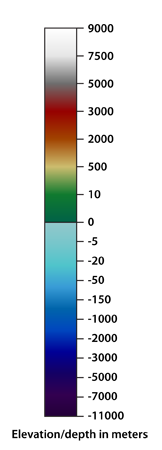
\includegraphics[width=0.2\paperwidth]{color.png}}
  \label{fig:Color}
\end{figure}
Source: \url{http://noaa.maps.arcgis.com/home/item.html?id=feb3c625dc094112bb5281c17679c769} 
Each vertex has its height. This Map of height indicates the height by color.

\item c. Base Support Module:
Create a frame around the mesh.
Find all vertices in directions: left, right, bottom \& top of mesh. Based on those vertices, draw a triangle to the point having the same coordinate but height = min(height) - 100

\item d. Rotate Module:
Rotate module catchs right-click and mouse movement, identify from/to points to rotate:

glRotatef of OpenGL is used to rotate
\begin{lstlisting}
glRotatef(xRot / 16.0, 1.0, 0.0, 0.0);
    	glRotatef(yRot / 16.0, 0.0, 1.0, 0.0);
    glRotatef(zRot / 16.0, 0.0, 0.0, 1.0);
\end{lstlisting}

\item e. Zoom Module:
Zoom module catchs scroll event of mouse to increase or decrease zoom level.
glOtho and glViewport functions are used to zoom
\begin{lstlisting}[breaklines=true]
int side = qMin(width, height);
glViewport(((width - side) / 2)*zoomByScale,((height - side) / 2)*zoomByScale, side*zoomByScale, side*zoomByScale);
glMatrixMode(GL_PROJECTION);
glLoadIdentity();
float aspectRatio = (float)width/(float)height;
glOrtho(-aspectRatio*zoomByScale, aspectRatio*zoomByScale, -1*zoomByScale, 1*zoomByScale, 1.0, 15.0);
glMatrixMode(GL_MODELVIEW);
\end{lstlisting}

\item f. Move Module:
Move module catchs left-click event and movement of mouse to identify the direction and distance.
\begin{lstlisting}
int distanceX = event->x() - lastPos.x();
        int distanceY = event->y() - lastPos.y();
        if (abs(distanceX) < abs(distanceY)) {
            y -= distanceY * 0.0001;
        } else {
            x += distanceX * 0.0001;
        }
\end{lstlisting}
\end{itemize}

\section{Bibliography}
\begin{enumerate}[{(1)}]

\item Digital elevation model. Retrieved from \url{https://en.wikipedia.org/wiki/Digital_elevation_model}. Wikipedia (2016, 9 April).

\item DEM (Digital Elevation Model) files. Retrieved from \url{http://vterrain.org/Elevation/dem.html}.Virtual Terrain Project (n.d.)

\item USGS DEM. Retrieved from \url{https://en.wikipedia.org/wiki/USGS_DEM}. Wikipedia (2016, March 10).

\item Digital Elevation Models - Data User Guide 5. Retrieved from \url{http://agdc.usgs.gov/data/usgs/geodata/dem/dugdem.pdf}. U.S. Geological Survey (1993).

\item Gridded Digital Elevation Model Product Specifications, edition 2.0. Retrieved from \url{http://www.geobc.gov.bc.ca/base-mapping/atlas/trim/specs/BC-DEM-specifications-2002-12.pdf}. Base Mapping and Geomatics Services Branch - Ministry of Sustainable Resource Management - Province of British Columbia (December 2002).

\item Terrain Tools - Importing USGS DEM data Example. Retrieved from \url{http://www.softree.com/Tips_Techniques/T-004-USGS-DEM/USGS_DEM.pdf}. Softree (n.d.).

\item Converting and Using SDTS Digital Elevation Model Data. Retrieved from \url{http://www.esri.com/news/arcuser/0799/webdata6.html}. Mike Price, ESRI (n.d.). 

\item What is SDTS?. Retrieved from \url{http://mcmcweb.er.usgs.gov/sdts/whatsdts.html}. U.S Geological Survey (n.d.). 

\item 
View the SDTS Document. Retrieved from \url{http://mcmcweb.er.usgs.gov/sdts/standard.html}. U.S. Geological Survey (n.d.).

\item Working with Digital Elevation Models and Digital Terrain Models in Arcmap 9. Retrieved from \url{http://www.lib.uwaterloo.ca/locations/umd/documents/WorkingWithDEM-DTMinArcMap.pdf}. David Findlay (June 2005).

\item DTED. Retrieved from \url{https://en.wikipedia.org/wiki/DTED}. Wikipedia (2016, 31 January).

\item Digital Terrain Elevation Data (DTED) - Part 1. Retrieved from \url{http://www.mission-planning.com/DTED_Part1.htm}. Paul, Pablo's Mission Planning Website (n.d.).

\item Digital Terrain Elevation Data [DTED]. Retrieved from \url{http://fas.org/irp/program/core/dted.htm}. Federation of American Scientists (n.d.).
 
\item Performance specification Digital terrain elevation data (DTED). Retrieved from \url{https://dds.cr.usgs.gov/srtm/version2_1/Documentation/MIL-PDF-89020B.pdf}. U.S. Department of Defense (2000, 23 May).

\item DTED files (Digital Terrain Elevation Data). Retrieved from \url{http://vterrain.org/Elevation/dted.html}. Virtual Terrain Project (n.d.).


\item The DIMAP format. Retrieved from \url{http://www.geo-airbusds.com/en/196-the-dimap-format}. Airbus Defense \& Space (n.d.).

\item Dimap structure. Retrieved from \url{http://www.spotimage.fr/dimap/spec/documentation/3.Dimap_structure.htm}. Airbus Defense \& Space (n.d.).

\item The IDE QtCreator. Retrieved from \url{http://www.qt.io/ide/}. The QtCompany (2016).

\item Richard S., Nicholas H., Graham S. and Benjamin Lipchak. OpenGL Superbible comprehensive tutorial and reference. 5th edition. Addison-Wesley, 2010. Print.
\end{enumerate}

\end{document}

